% Compile with: pdflatex (run TWICE to resolve cross-references)
\documentclass[11pt]{article}
\usepackage[letterpaper, margin=1in, top=0.9in, bottom=0.9in]{geometry}
\usepackage[T1]{fontenc}
\usepackage[utf8]{inputenc}
\usepackage{mathpazo}
\usepackage{microtype}
\usepackage[htt]{hyphenat}
\usepackage{amsmath}
\usepackage{amssymb}
\usepackage{titlesec}
\usepackage{enumitem}
\usepackage{booktabs}
\usepackage{graphicx}
\usepackage{caption}
\usepackage{float}
\usepackage[authoryear,round]{natbib}
\usepackage{hyperref}
\usepackage{xurl}
\usepackage{setspace}
\usepackage{xcolor}
\usepackage{mdframed}
\makeatletter
\renewcommand\@biblabel[1]{}
\makeatother

\titleformat{\section}{\normalfont\large\bfseries}{\thesection.}{0.6em}{}
\titleformat{\subsection}{\normalfont\normalsize\bfseries}{\thesubsection.}{0.5em}{}
\titlespacing*{\section}{0pt}{1.2em}{0.4em}
\titlespacing*{\subsection}{0pt}{0.9em}{0.25em}

\captionsetup{font=small, skip=4pt}

\setlength{\parskip}{0.5em}
\setlength{\parindent}{0pt}
\setlength{\emergencystretch}{3em}
\setlist{itemsep=0.2em, topsep=0.3em, partopsep=0pt, leftmargin=1.5em}

% Box for instructor feedback
\newmdenv[
  linewidth=0.5pt,
  linecolor=black!40,
  backgroundcolor=black!4,
  skipabove=0.4em,
  skipbelow=0.3em,
  innerleftmargin=8pt,
  innerrightmargin=8pt,
  innertopmargin=5pt,
  innerbottommargin=5pt
]{feedbackbox}

\begin{document}

% ─────────────────────────── TITLE ─────────────────────────────────────────
\begin{center}
  {\large\bfseries Epic Games Store Giveaways: Causal Effect on Steam Player Engagement}\\[0.4em]
  {\small Nicholas Liu \quad|\quad 14.33 --- Assignment 7}
\end{center}

\vspace{0.5em}
\hrule
\vspace{0.8em}

% ═══════════════════════════════════════════════════════════════════════════
\section{Revised Versions of A5 and A6}
% ═══════════════════════════════════════════════════════════════════════════

The following subsections revise each component from Assignments 5 and 6, 
relevant feedback from Theo is quoted in shaded boxes, followed by a brief response 
and the revised text.

% ─────────────────────────────────────────────────────────────────────────
\subsection{(a) Data Sources}
% ─────────────────────────────────────────────────────────────────────────

\textit{No specific feedback received here.}

\textbf{Epic Games Store giveaway history.}
I obtained a Kaggle dataset \citep{dongre2025} recording every free game
offered through the Epic Games Store from December 2018 through 2025,
comprising 541 giveaway events corresponding to 471 unique titles.
The remaining 70 events are repeat appearances of titles already given away.
Nine titles had the ``(repeat)'' suffix incorrectly applied to their
\textit{first} appearance in the source file; these were manually corrected.
Repeats cluster in two patterns: \textit{proximate} (second event within 12
months of the first, most commonly during Epic's annual holiday batches) and
\textit{distant} ($>$12 months).

\textbf{SteamCharts monthly player data.}
For each EGS title matched to a Steam App ID, I scraped monthly average and
peak concurrent player counts from \texttt{steamcharts.com}. SteamCharts
renders historical tables server-side, so standard HTTP requests suffice.
The overall panel spans July 2012 through February 2026; each game's time
series begins near its Steam release date. The median game has 88 months
of data.

\textbf{Merge pipeline.}
Matching Epic game names to Steam App IDs requires reconciling inconsistent
titling (subtitles, punctuation, edition suffixes). I used RapidFuzz fuzzy
string matching, which auto-matched 413 of 471 unique names; the remaining
58 received manual review, of which 50 resolved to a valid Steam App ID and
8 were confirmed absent from Steam (5 Epic exclusives and 3 placeholder
entries). Thirteen matched entries returned HTTP 500 errors from SteamCharts
and were excluded.

\textbf{Final panel.}
The assembled dataset contains 38{,}642 game--month observations across
446 games, spanning July 2012 through February 2026. Of these 446 games,
421 have SteamCharts data covering their treatment month and 336 have a
full $[-12,+12]$ event window.

% ─────────────────────────────────────────────────────────────────────────
\subsection{(b) Proposed Empirical Test}
% ─────────────────────────────────────────────────────────────────────────

\begin{feedbackbox}
\small\textit{``Is there a reason you are not including the games that were
never given away as controls? \ldots{} Right now, from my understanding,
your specification is a no-never-treated event study, and the lack of never
treated units introduces some complexity. You might need to exclude at least
two periods to avoid collinearity with your time fixed effects, and because
of that, you'd need to add in the assumption that the omitted periods can be
pooled. If you add never treated controls (or do a stacked event study that
essentially creates never treated controls), you avoid some of that
complexity. Also, are you planning to only use the observations in $[-12,12]$
or will you be binning your event study at $-12+$ and $12+$?''}
\end{feedbackbox}

\textbf{Response.}

\textit{Never-treated controls.}
I considered adding never-treated controls but ultimately did not construct an
external never-treated pool for two reasons. First, there is no principled,
non-selective sampling frame for choosing which of the approximately 50{,}000
non-EGS Steam titles to include; any genre-, vintage-, or popularity-based
criterion risks assembling a control group whose trajectories happen to be
stable, biasing the comparison. Second, the not-yet-treated design sidesteps
this problem because every game in my sample is eventually treated by Epic,
so the control group at any point is drawn from the same population of
EGS-eligible titles.

Following your suggestion, I implemented stacked DiD \citep{cengiz2019} 
and constructed cohort-specific
balanced panels with \textit{only} not-yet-treated games as controls within
each cohort stack, then estimated TWFE with cohort fixed effects. This
achieves the identification benefit of a never-treated group (clean controls,
no negative-weighting bias) without requiring an external sample. 

\textit{Collinearity and omitted periods.}
Because I have 80 treatment cohorts distributed across 80 distinct calendar
months (December 2018 through late 2025), at any calendar
month $t$, the panel contains games at a wide range of event-times (recently
treated, approaching treatment, and far from it). This staggered
structure means the calendar-month fixed effects and event-time dummies are
not collinear, and omitting only the single reference period $k = -1$ should be
sufficient for identification. 

\textit{Binning vs.\ restricting.}
I use boundary-bin clipping: observations with $k < -12$ are binned into the
$k = -12$ cell, and observations with $k > 12$ into $k = 12$. This retains
all 446 games rather than the 336 with a full $[-12,+12]$ window. Interior
estimates at $k \in [-11, 11]$ are unaffected; the boundary-bin estimates at
$k = \pm 12$ pool over all periods beyond the window and should be read as
averages. A robustness check restricted to the 336-game full-window subsample
yields qualitatively identical results.

\textbf{Revised specification.}
The primary specification is a two-way fixed-effects (TWFE) event-study
regression on the full unbalanced game--month panel:
\begin{equation}
\label{eq:pooled}
\ln(y_{it} + 1) = \alpha_i + \gamma_t +
  \sum_{\substack{k \in [-12,\,12] \\ k \neq -1}}
  \theta_k \cdot \mathbf{1}[\tilde{k}_{it} = k]
  + \varepsilon_{it}
\end{equation}
where $\alpha_i$ are game fixed effects, $\gamma_t$ are calendar-month fixed
effects, and $\tilde{k}_{it} = \text{clip}(k_{it},\,-12,\,12)$ is the
clipped event-time indicator. The omitted category is $k = -1$. Standard
errors are clustered at the game level.

As robustness checks I compare this TWFE estimate to three complementary
estimators that restrict controls to not-yet-treated games: (i) LP-DiD
\citep{dube2023}, which estimates each period-$k$ effect using a separate
local projection on not-yet-treated controls; (ii) stacked DiD
\citep{cengiz2019}, which constructs cohort-specific balanced panels with
not-yet-treated controls and estimates TWFE with cohort fixed effects; and
(iii) Callaway--Sant'Anna cohort ATTs \citep{callaway2021}, aggregated
across cohorts weighted by cohort size.

% ─────────────────────────────────────────────────────────────────────────
\subsection{(c) Assumptions Required for Validity}
% ─────────────────────────────────────────────────────────────────────────

\textit{No specific feedback received here.}

\textbf{Parallel trends.} In the absence of treatment, log player counts
across cohorts would have followed the same time path after conditioning on
game and calendar-month fixed effects. This requires that Epic's curation
team does not systematically select games at particular inflection points in
their Steam lifecycle. There is, however, reason to believe this assumption
is at least partially violated: the pre-period event-study coefficients for
$k \in [-12, -1]$ trace a negative slope, consistent with Epic preferentially
selecting titles already in lifecycle decline. This selection concern is the
central identification caveat of the design.

\textbf{No anticipation.} Player behavior does not shift before the giveaway
month. Epic typically announces the following week's free game only one week
ahead, making systematic pre-treatment anticipation on Steam unlikely.

% ─────────────────────────────────────────────────────────────────────────
\subsection{(d) Thoughts on Testing the Assumptions}
% ─────────────────────────────────────────────────────────────────────────

\textit{No specific feedback received here.}

\textbf{Pre-trend Wald test.} I test $H_0: \theta_k = 0$ for all
$k \in [-12, -2]$ jointly using a Wald test. A failure to reject supports
parallel trends (necessary but not sufficient). The full-sample test yields
$\chi^2 = 21.77$ ($df = 11$, $p = 0.026$), a marginal rejection. For the
high-traffic subsample (215 games above the pre-treatment median), the test
yields $p = 0.589$, consistent with cleaner identification for more popular
titles where lifecycle noise is lower.

\textbf{Popularity-stratified analysis.} Splitting the sample at the median
pre-treatment player count diagnoses whether the pooled result is driven by
noise in the lower tail. High-traffic games show larger, more precisely
estimated contemporaneous spikes and cleaner pre-trends.

\textbf{Randomization placebo.} I permute treatment dates across all 446
games 200 times and compare the actual $|\hat{\theta}_0|$ to the permutation
null distribution. The permutation $p$-value is $p < 0.001$: the actual
$|\hat{\theta}_0| = 0.101$ exceeds the 95th percentile of the permutation null
(0.038).

\textbf{Estimator comparison.} Agreement across TWFE, LP-DiD, stacked DiD,
and Callaway--Sant'Anna on the qualitative two-phase pattern supports internal
validity; the quantitative spread across estimators informs the plausible
range of the causal effect.

% ─────────────────────────────────────────────────────────────────────────
\subsection{(e) Problems Anticipated}
% ─────────────────────────────────────────────────────────────────────────

\begin{feedbackbox}
\small\textit{``I wonder if you have any special interest in games with
repeated giveaways. If they make up a tiny share of your sample and aren't
particularly interesting, I would probably just exclude them.''}
\end{feedbackbox}

\textbf{Response.}
Repeat giveaways account for only 2\% of game--month
observations and the repeat-event coefficient is $\hat{\delta} = 0.0001$
($p = 0.999$), statistically and economically indistinguishable from zero.
A clean-sample robustness check that entirely drops all 30 proximate-repeat
games (second giveaway within 12 months of the first, $<$7\% of games)
yields main estimates nearly identical to the full sample.

\textbf{Revised text.}

\textbf{No never-treated group.} All 446 games are eventually treated, so
identification rests entirely on timing variation across cohorts. If earlier
cohorts (2019--2020) differ systematically from later cohorts (2022--2025)
in unobserved ways, parallel trends is harder to defend. The stacked DiD and
Callaway--Sant'Anna estimators partially mitigate this by restricting controls
to not-yet-treated games within each cohort.

\textbf{Selection of games in lifecycle decline.} The pre-period event-study
coefficients trace a negative slope, consistent with Epic preferentially
selecting titles already on a downward Steam trajectory. Much of the observed
post-giveaway decline may therefore reflect the continuation of a pre-existing
trend rather than a causal consequence of the giveaway. The LP-DiD estimate
should be interpreted as an upper bound on the true causal substitution effect.

\textbf{Noisy low-player-count games.} Of the 446 games, 101 have a
pre-treatment median below 10 concurrent players. The log transformation
amplifies proportional noise for near-zero values; the popularity-stratified
analysis isolates this concern.

\textbf{Repeat giveaways (resolved).} The 30 proximate-repeat games (second
event within 12 months) are handled via a scalar $\text{repeat\_event}_{it}$
indicator. The estimate $\hat{\delta} \approx 0$ confirms no contamination;
excluding these games entirely leaves main estimates unchanged.

\textbf{DLC/bundle mapping.} Fifteen events distributed DLC or in-game
content rather than the base game. Mapping these to the base game's Steam
App ID likely attenuates the estimated treatment effect for those
observations.

\textbf{Player counts vs.\ purchases.} SteamCharts reports concurrent
players, not purchases or unique installs. The giveaway effect on purchasing
may be larger or differently timed than the player-count effect estimated
here.

% ─────────────────────────────────────────────────────────────────────────
\subsection{(f) Brief Review of Related Literature}
% ─────────────────────────────────────────────────────────────────────────

\begin{feedbackbox}
\small\textit{``On the paper side, I'd try to explain how your analysis
differs from Clarkson's.''}
\end{feedbackbox}

\textbf{Response.}
The revised literature review now includes a dedicated paragraph
explicitly distinguishing this paper from Clarkson along three dimensions:
the length of the event-study window (twelve months versus contemporaneous
only), the use of pre-period path to document selection on lifecycle decline,
and sample breadth (446 matched EGS titles versus a curated subset).

\textbf{Revised literature review.}

\textbf{Cross-platform spillovers and platform competition.}
The most directly related work is \citet{clarkson2025}, a doctoral
dissertation whose second chapter quasi-experimentally studies cross-platform
spillover effects of gaming platform giveaways. Using Steam player traffic
data, Clarkson finds that games given away by a competing platform (Epic) see
Steam traffic increase by more than 24\%. He also documents that word-of-mouth
and Steam review activity increase significantly during these promotions, and
that spillover effects are larger for games that leverage Steam-exclusive
features (friend lists, achievements, community hubs).

The present paper differs from Clarkson's in three key respects. First, and
most substantially, Clarkson's analysis focuses on the short-run
contemporaneous effect; this paper estimates the full twelve-month
post-treatment trajectory, documents the systematic reversal below
pre-giveaway baseline that prior work has not characterized, and employs
multiple heterogeneous-treatment-robust estimators (LP-DiD, stacked DiD,
Callaway--Sant'Anna) to bound the plausible range of the causal effect.
Second, by tracking the pre-period event-study path, this paper provides
evidence that the post-giveaway decline reflects selection on lifecycle
decline rather than causal substitution alone, a mechanism invisible to a
contemporaneous-only design. Third, the sample matches the full EGS giveaway
catalogue (446 titles matched to Steam, 2018--2025) rather than a curated
subset, enabling a broader characterization of the average effect.

More broadly, the question fits into the literature on platform competition
and multi-homing in two-sided markets \citep{rochet2003}. When two platforms
serve the same user base (as Steam and EGS do for PC gamers), a free
promotion on one platform may reallocate engagement rather than expand the
aggregate market.

\citet{tudon2022} estimates direct network effects on Steam and finds a
0.13\% own-demand increase per 1\% increase in friends' demand. This
social-multiplier channel provides a mechanism for the advertising effect:
by expanding the addressable player community, a free copy on a rival
platform may activate network complementarities that benefit the incumbent.

\citet{nabil2025} find that Steam significantly outperforms EGS on content
variety and ease of use, and that Epic's free game program attracts users
without closing the satisfaction gap. This is consistent with a world where
Steam's incumbency advantage is durable: players who obtain a game via Epic
may still wish to engage with Steam's ecosystem for reviews, achievements,
and community features.

Methodologically, the backbone draws on \citet{callaway2021} for
cohort-robust staggered DiD, \citet{cengiz2019} for stacked DiD, and
\citet{dube2023} for LP-DiD.

% ─────────────────────────────────────────────────────────────────────────
\subsection{(g) Summary Statistics: Table and Figure}
% ─────────────────────────────────────────────────────────────────────────

\textit{No specific feedback received here.}

Table~\ref{tab:sumstats} presents summary statistics for the key variables.
Raw player counts are highly right-skewed: the mean monthly average of
1{,}584 players is more than 24 times the median of 65 players, reflecting a
distribution dominated by long-tail indie titles with occasional blockbusters
(e.g., GTA~V, Destiny~2). The log-transformed outcome is far better behaved
(mean 4.43, SD 2.36), as intended. The repeat-event indicator equals 1 in
only 2\% of game--month observations.

\begin{table}[H]
\centering\small
\caption{Summary statistics: Epic giveaway panel}
\label{tab:sumstats}
\begin{tabular}{lrccccc}
\toprule
Variable & $N$ & Mean & SD & Min & Median & Max \\
\midrule
Avg.\ concurrent Steam players (monthly) & 38,642 & 1,583.9 & 7,444.0 & 0.00 & 65.2 & 270,553 \\
Peak concurrent Steam players (monthly)  & 38,642 & 3,214.1 & 14,861.2 & 0 & 171 & 527,652 \\
$\ln(\texttt{avg\_players}+1)$ [outcome] & 38,642 & 4.43 & 2.36 & 0.00 & 4.19 & 12.51 \\
Repeat-giveaway window indicator (0/1)   & 38,642 & 0.02 & 0.15 & 0 & 0 & 1 \\
\midrule
Months of SteamCharts data per game & 446 & 86.6 & 41.1 & 1 & 88 & 163 \\
\bottomrule
\end{tabular}
\medskip

\noindent\small\textit{Notes:} Game--month panel, 446 games, July 2012--February 2026.
  Player counts are in raw players as reported by SteamCharts.com.
  The outcome variable $\ln(\texttt{avg\_players}+1)$ uses a $+1$ offset to
  accommodate months with zero reported players.
  The repeat-giveaway window indicator equals 1 in months falling within
  12 months after a game's second (or later) Epic giveaway.
  The bottom row is game-level ($N = 446$ unique games).
\end{table}

Figure~\ref{fig:outcome} presents two panels characterizing the outcome
variable. The left panel shows overlaid density histograms of
$\ln(\texttt{avg\_players}+1)$ for pre-giveaway ($k < 0$) and post-giveaway
($k \geq 0$) months. Both distributions are roughly unimodal with a long
right tail; the large mass near zero reflects the many low-traffic titles.
The right panel plots the unconditional mean of the outcome at each event-time
$k \in [-12, 12]$: the pre-period mean is approximately flat, providing
preliminary (unconditional) support for the parallel trends assumption, and a
sharp uptick is visible at $k = 0$ with partial persistence into $k = 1$.

Figure~\ref{fig:desc} provides three additional descriptive panels. Panel~(a)
shows the roughly bimodal pre-treatment distribution of log players across
games, with a large cluster of low-traffic titles and a smaller cluster of
popular ones. Panel~(b) shows that treatment cohorts are broadly evenly
distributed across 2019--2023, providing the timing variation needed for
staggered DiD. Panel~(c) shows that approximately 10\% of games in most
cohort years have a proximate repeat giveaway.

\begin{figure}[H]
\centering
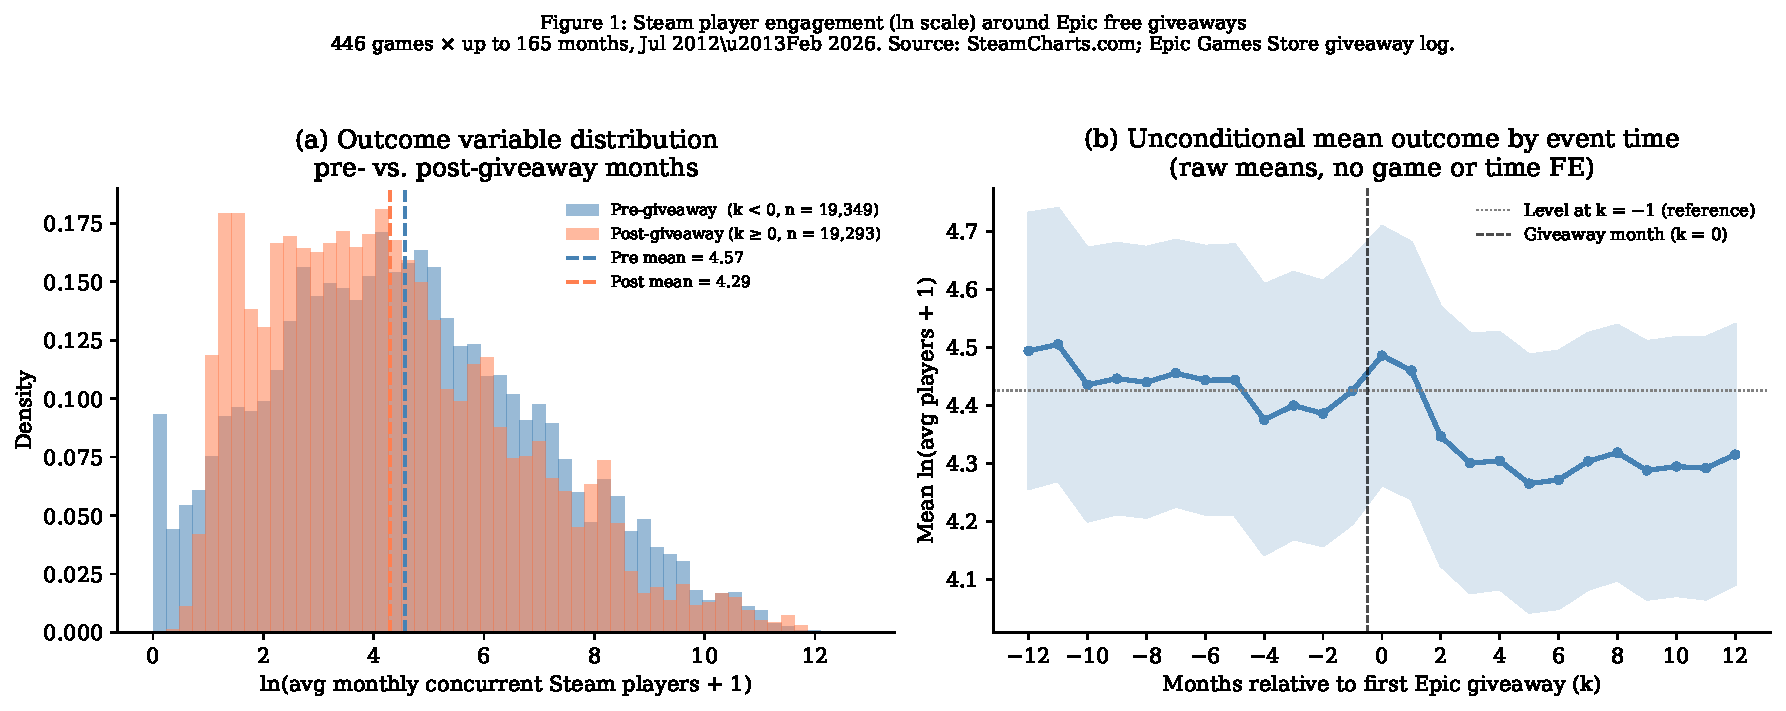
\includegraphics[width=0.88\linewidth]{../output/fig_outcome_histogram.pdf}
\caption{Steam player engagement (log scale) around Epic free giveaways.
  \textbf{Left:} Density histogram of $\ln(\texttt{avg\_players}+1)$ for
  pre-giveaway months ($k < 0$, blue) and post-giveaway months
  ($k \geq 0$, orange), pooled across all 446 games.
  \textbf{Right:} Unconditional mean (with 95\% CI) of the outcome by
  event-time $k \in [-12,12]$; the dashed vertical line marks the giveaway
  month ($k = 0$). Both panels use 38,642 game--month observations.
  \textit{Source:} SteamCharts.com; Epic Games Store giveaway log \citep{dongre2025}.}
\label{fig:outcome}
\end{figure}

\begin{figure}[H]
\centering
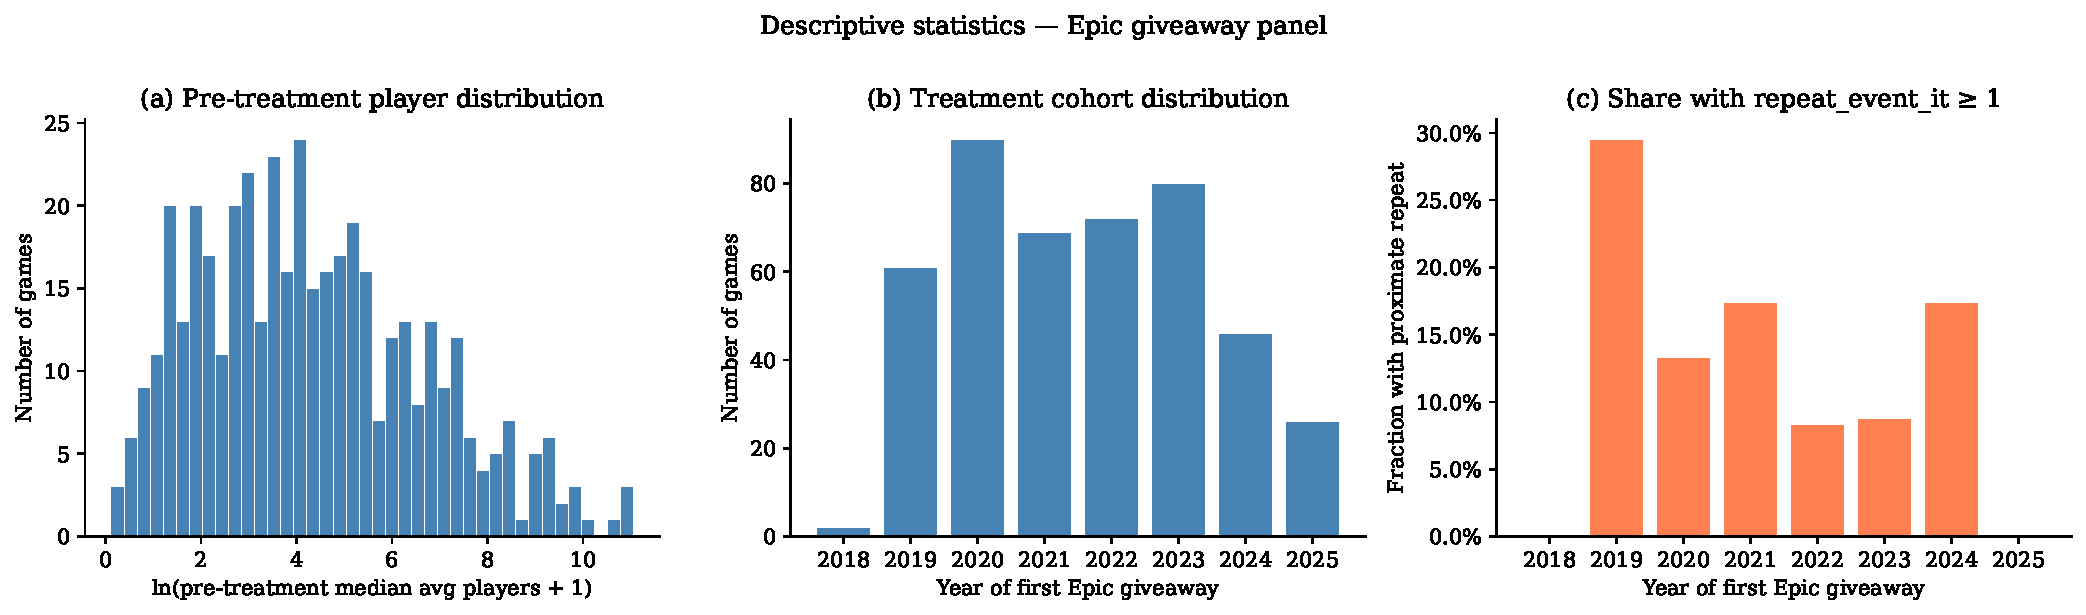
\includegraphics[width=0.88\linewidth]{../output/fig_descriptives.pdf}
\caption{Panel structure and descriptive statistics.
  \textbf{(a)} Histogram of $\ln(\text{pre-treatment median avg players} + 1)$
  across 446 games.
  \textbf{(b)} Number of games with first Epic giveaway in each calendar year
  (2018--2025).
  \textbf{(c)} Fraction of games with a proximate repeat giveaway (second
  event within 12 months of first) by cohort year.
  \textit{Source:} SteamCharts.com; Epic Games Store giveaway log \citep{dongre2025}.}
\label{fig:desc}
\end{figure}

% ═══════════════════════════════════════════════════════════════════════════
\section{Paper Outline}
% ═══════════════════════════════════════════════════════════════════════════

\begin{enumerate}[leftmargin=2em]
  \item \textbf{Introduction}: Motivating anecdote (Blood West case, Reddit thread);
    research question (does an EGS giveaway increase or decrease Steam engagement?);
    preview of two-phase finding (short-run spike, medium-run reversal); brief
    description of identification strategy and data; contributions.

  \item \textbf{Literature Review}
    \begin{itemize}
      \item Cross-platform spillovers: Clarkson (2025) contemporaneous effect;
        differences from present paper
      \item Network effects and social multipliers: Tudon (2022)
      \item Platform satisfaction and incumbency: Nabil \& Ariatmanto (2025)
      \item Staggered DiD methodology: Callaway \& Sant'Anna (2021),
        Dub\'e et al.\ (2023) LP-DiD, Cengiz et al.\ (2019) stacked DiD
    \end{itemize}

  \item \textbf{Data}
    \begin{itemize}
      \item Epic Games Store giveaway history (Kaggle, 541 events, 471 titles)
      \item SteamCharts monthly player data (scraping, panel structure)
      \item Merge pipeline (RapidFuzz matching, 446-game final panel)
      \item Summary statistics; data limitations
    \end{itemize}

  \item \textbf{Empirical Method}
    \begin{itemize}
      \item Identification strategy (not-yet-treated design, staggered timing)
      \item Pooled TWFE specification; identification in no-never-treated design;
        boundary-bin clipping
      \item Separated specification: first vs.\ repeat giveaways
      \item Robustness estimators: LP-DiD, stacked DiD, Callaway--Sant'Anna
      \item Additional checks: popularity stratification, randomization placebo
    \end{itemize}

  \item \textbf{Results}
    \begin{itemize}
      \item Main TWFE event study: spike at $k=0$, reversal from $k=2$
      \item Pre-trend Wald test (full sample $p=0.026$; high-traffic $p=0.589$)
      \item Estimator comparison: TWFE, LP-DiD, stacked DiD (quantitative spread;
        qualitative agreement)
      \item Separated specification: $\hat{\delta} \approx 0$ for repeats
      \item Popularity-stratified analysis
      \item Callaway--Sant'Anna cohort ATTs
      \item Randomization placebo ($p < 0.001$)
    \end{itemize}

  \item \textbf{Discussion}
    \begin{itemize}
      \item Contemporaneous spike: advertising mechanism; comparison to Clarkson
      \item Medium-run reversal: selection on lifecycle decline (primary explanation);
        direct substitution; counterfactual demand exhaustion
      \item Null repeat-giveaway effect
      \item Platform strategy implications for developers and Epic
      \item Limitations: no never-treated group, selection concern, player counts
        vs.\ purchases, DLC mapping, genre heterogeneity
    \end{itemize}

  \item \textbf{Conclusion}: Summary of two-phase finding; primary mechanism
    (lifecycle selection $>$ causal substitution); implications for platform strategy;
    directions for future work (single- vs.\ multiplayer split; Steam sales data;
    Epic-side engagement data).
\end{enumerate}

% ═══════════════════════════════════════════════════════════════════════════
\section{Results}
% ═══════════════════════════════════════════════════════════════════════════

\subsection{Main TWFE Event Study}

Table~\ref{tab:coefs} reports selected TWFE event-study coefficients
($\hat{\theta}_k$, Equation~\eqref{eq:pooled}) with standard errors clustered
by game. The pre-period coefficients for $k \in [-5, -2]$ are small and
individually insignificant, consistent with approximate parallel trends over
the near-term pre-window. In the giveaway month ($k = 0$), the coefficient
is $\hat{\theta}_0 = 0.101$ (SE $= 0.022$, $p < 0.001$), implying
approximately a 10.6\% increase in monthly average concurrent Steam players.

The spike is short-lived. By $k = 2$ the coefficient turns negative
($-0.063$, $p = 0.005$), and the decline accelerates through the full window.
By $k = 12$ the estimated coefficient is $-0.267$ (SE $= 0.053$,
$p < 0.001$), implying approximately 23\% fewer players relative to the
pre-giveaway baseline. The $R^2$ of the game--month regression is 0.884
(within $R^2 = 0.008$), confirming that most variation in log players is
accounted for by game-level and time fixed effects, with the event-study
coefficients capturing the residual treatment effect.

\begin{table}[H]
\centering\small
\caption{Selected TWFE event-study coefficients (pooled specification,
  Eq.~\eqref{eq:pooled})}
\label{tab:coefs}
\begin{tabular}{rrcl}
\toprule
Event time $k$ & Estimate & SE & $p$-value \\
\midrule
$-5$ &  $\phantom{-}0.005$ & 0.025 & 0.833 \\
$-4$ &  $-0.003$ & 0.024 & 0.915 \\
$-3$ &  $-0.009$ & 0.025 & 0.710 \\
$-2$ &  $-0.011$ & 0.022 & 0.608 \\
\midrule
$\phantom{-}0$ & $\mathbf{0.101}^{***}$ & 0.022 & $<$0.001 \\
$\phantom{-}1$ & $0.045^{*}$ & 0.022 & 0.047 \\
$\phantom{-}2$ & $-0.063^{**}$ & 0.023 & 0.005 \\
$\phantom{-}3$ & $-0.097^{***}$ & 0.024 & $<$0.001 \\
$\phantom{-}6$ & $-0.160^{***}$ & 0.027 & $<$0.001 \\
$\phantom{-}9$ & $-0.178^{***}$ & 0.031 & $<$0.001 \\
$12$ & $-0.267^{***}$ & 0.053 & $<$0.001 \\
\bottomrule
\end{tabular}
\medskip

\noindent\small\textit{Notes:} Dependent variable: $\ln(\texttt{avg\_players}+1)$.
  Game and calendar-month fixed effects;
  standard errors clustered by game ($N = 38{,}641$; 446 games).
  Omitted period: $k = -1$. $R^2 = 0.884$; within $R^2 = 0.008$.
  $^{*}p<0.05$, $^{**}p<0.01$, $^{***}p<0.001$.
\end{table}

\subsection{Estimator Comparison}

Figure~\ref{fig:compare} overlays the TWFE, LP-DiD \citep{dube2023}, and
stacked DiD \citep{cengiz2019} event-study estimates. All three estimators
agree on the qualitative two-phase pattern (a positive spike at $k = 0$
followed by a sustained and statistically significant reversal), but they
differ quantitatively in ways that are informative about the range of the
true causal effect.

At $k = 0$, TWFE yields 0.101 (95\% CI [0.058, 0.144]), LP-DiD yields 0.131
(CI [0.088, 0.173]), and stacked DiD yields 0.047 (CI [0.032, 0.063]). The
stacked DiD estimate, which constructs cohort-balanced panels and uses only
not-yet-treated controls, is likely the most conservative and is the
preferred estimate of the contemporaneous effect ($\approx$5\% increase).
TWFE and LP-DiD exceed stacked DiD, consistent with cohort-composition bias
in the former.

In the medium run, all three estimators show statistically significant
declines from $k = 3$ or $k = 5$ onward. At $k = 10$, the estimates span
from LP-DiD ($-0.121$, CI [$-0.191$, $-0.051$]) to stacked DiD ($-0.164$,
CI [$-0.201$, $-0.127$]) to TWFE ($-0.199$, CI [$-0.259$, $-0.138$]). The
LP-DiD estimate, which conditions most directly on pre-treatment trends by
using only not-yet-treated controls at each period, provides the most
conservative medium-run estimate and should be interpreted as an upper bound
on the true causal substitution effect, because the pre-period negative slope
indicates that treated games were already declining before the giveaway.

The pre-period path ($k \in [-12, -1]$) traces a downward slope across all
three estimators, providing the most direct evidence of Epic's selection of
titles already in lifecycle decline. This pre-existing trajectory likely
accounts for a meaningful share of the post-giveaway reversal: the
approximately 0.08 log-point gap between TWFE and LP-DiD at $k = 10$
reflects the portion of the observed reversal that LP-DiD attributes to this
pre-existing selection rather than to the giveaway itself.

\begin{figure}[H]
\centering
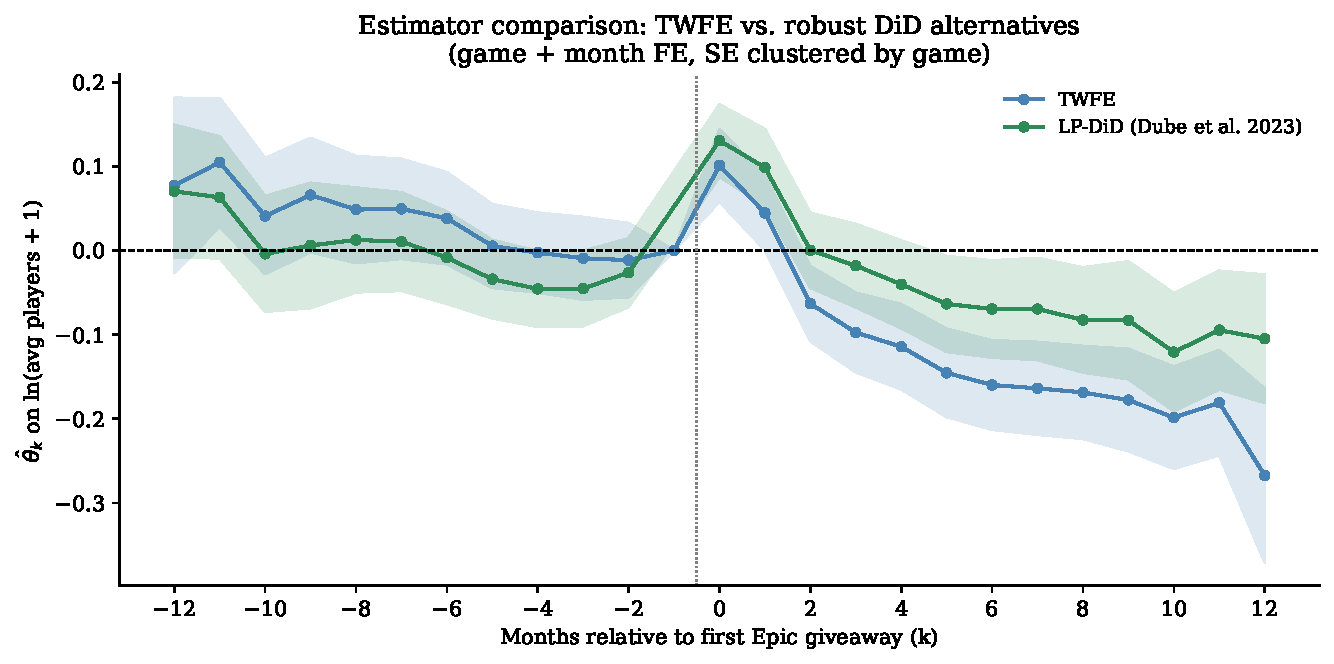
\includegraphics[width=0.88\linewidth]{../output/fig_estimator_comparison.pdf}
\caption{Event-study estimates: TWFE, LP-DiD \citep{dube2023}, and stacked
  DiD \citep{cengiz2019}. Outcome: $\ln(\texttt{avg\_players}+1)$.
  LP-DiD uses only not-yet-treated controls at each
  period $k$ independently. Stacked DiD constructs cohort-specific balanced
  panels with not-yet-treated controls, weighted by $1/\text{number of stacks
  per game}$. Shaded bands are 95\% confidence intervals (standard errors
  clustered by game). Reference period $k = -1$. $N = 38{,}641$ game--month
  observations; 446 games.
  }
\label{fig:compare}
\end{figure}

\subsection{Economic Significance and Developer Calculus}

\subsubsection*{Developer calculus}

The developer calculus is cleaner than it first appears. The pre-existing
lifecycle decline is irrelevant to the decision: it would have happened
regardless of whether the developer signs the deal. The substitution
component is also not a net developer cost: a player who migrates from
Steam to Epic is still playing the game, and Epic's 12\% revenue cut is
more favorable than Steam's 30\%. The deal therefore reduces to two
clearly positive terms: the licensing fee and the advertising spike.

The advertising benefit is real. We estimate a $+5$--$14\%$ Steam
engagement boost at $k = 0$ depending on estimator. \citet{clarkson2025}
shows Steam reviews spike alongside concurrent players during giveaways,
feeding Steam's recommendation algorithm and generating downstream sales
beyond our 12-month window. The Blood West case \citep{frvr2026}, a
200\% Steam sales spike from a single EGS giveaway, suggests the
purchase-conversion effect can be far larger than the engagement effect
we estimate. For developers, accepting the EGS deal is almost always
the correct decision.

\subsubsection*{Should Steam be concerned about EGS giveaways?}

No. The giveaway program is a net positive for Steam. The $k = 0$ spike
accrues directly to Steam in the form of increased concurrent players,
store page traffic, and reviews. Steam's position as the primary discovery
and community layer for PC gaming means that the media coverage generated
by an EGS giveaway announcement funnels curious players toward Steam, not
away from it. The medium-run concurrent-player decline is mostly pre-existing
lifecycle decline in titles that were already losing Steam players before
the giveaway; Epic is not causing Steam games to lose players, it is
selecting games that were already losing them. The residual causal
substitution component reflects marginal players on declining titles, not
the engaged users who sustain Steam's social ecosystem. The evidence that
the advertising effect occurs on Steam and that even free distribution
through a rival platform drives players to Steam's community infrastructure
is consistent with Steam's competitive moat being durable.

\subsubsection*{Does the giveaway program benefit Epic?}

The more interesting and harder question is whether the giveaway program
benefits Epic. Epic bears the full licensing cost but receives none of
the Steam advertising benefit our results document: the $k = 0$ spike is
in Steam concurrent players, Steam reviews increase, and the discovery
activity generated by the announcement happens on Steam's platform.
What Epic plausibly gains instead is EGS user acquisition: players who
install the launcher and become habitual EGS shoppers. Whether this
actually happens is not answerable with our data; we observe Steam
engagement but have no window into EGS-side behavior. Our results do,
however, raise a pointed question: if the primary measurable effect of
Epic's giveaway spending is to advertise games on Steam, Epic is paying
licensing fees to benefit a competitor's platform. Whether durable EGS
user acquisition offsets this is the most important open question for
evaluating the program's long-run strategic rationale.

\clearpage

% ─────────────────────────── BIBLIOGRAPHY ────────────────────────────────
\begin{thebibliography}{Callaway and Sant'Anna (2021)}
\setlength{\itemsep}{0.5em}

\bibitem[Callaway and Sant'Anna(2021)]{callaway2021}
Callaway, B.\ and Sant'Anna, P.H.C.\ (2021). ``Difference-in-Differences
with Multiple Time Periods.'' \textit{Journal of Econometrics}, 225(2),
200--230.

\bibitem[Cengiz et al.(2019)]{cengiz2019}
Cengiz, D., Dub\'{e}, A., Lindner, A., and Zipperer, B.\ (2019). ``The
Effect of Minimum Wages on Low-Wage Jobs.'' \textit{Quarterly Journal of
Economics}, 134(3), 1405--1454.

\bibitem[Clarkson(2025)]{clarkson2025}
Clarkson, T.C.\ (2025). ``Essays on Platform Operations.'' Doctoral
dissertation, Moore School of Business, University of South Carolina.

\bibitem[Dongre(2025)]{dongre2025}
Dongre, P.\ (2025). ``Epic Games Free Giveaway History 2018--2025.''
Kaggle dataset.

\bibitem[Dub\'{e} et al.(2023)]{dube2023}
Dub\'{e}, A., Girardi, D., Jord\`{a}, O., and Taylor, A.M.\ (2023).
``A Local Projections Approach to Difference-in-Differences Event Studies.''
NBER Working Paper No.\ 31184.

\bibitem[Nabil and Ariatmanto(2025)]{nabil2025}
Nabil, M.\ and Ariatmanto, D.\ (2025). ``Analysis of User Satisfaction and
Preferences in Choosing a Digital Game Platform.'' \textit{G-Tech: Jurnal
Teknologi Terapan}, 9(3), 1166--1175.

\bibitem[Rochet and Tirole(2003)]{rochet2003}
Rochet, J.-C.\ and Tirole, J.\ (2003). ``Platform Competition in Two-Sided
Markets.'' \textit{Journal of the European Economic Association}, 1(4),
990--1029.

\bibitem[Tud\'on(2022)]{tudon2022}
Tud\'on, J.\ (2022). ``Distilling Network Effects from Steam.''
\textit{Quantitative Marketing and Economics}, 20, 293--312.

\bibitem[FRVR Blog(2026)]{frvr2026}
FRVR Blog (2026). ``Epic Game Store's Free Giveaways Just Cause a Huge
Spike in Steam Sales, Reveals New Blood CEO\@.'' \textit{FRVR Blog},
January 20, 2026.

\end{thebibliography}

\vspace{0.5em}
\noindent\textit{Note on AI usage: I used AI to assist with drafting and
formatting this document in \LaTeX.}

\end{document}
